\section{Modelo proposto}

O classificador recebe uma imagem e prevê uma das cinco classes do conjunto
de dados. Foram avaliadas as arquiteturas ResNet-18, ResNet-50,
EfficientNet-B0, MobileNetV3-Large e ConvNeXt-Tiny com pesos pré-treinados
no ImageNet. Em cada arquitetura, a última camada foi substituída por
uma camada linear com cinco saídas. Também foi treinada uma ResNet-18
com pesos iniciais aleatórios para comparar o efeito do pré-treinamento.
A Fig.~\ref{fig:fluxo} resume o desenho experimental.

% Adicione \usepackage{graphicx} ao preâmbulo do artigo.
% O recorte conserva o diagrama e remove a legenda e o número de página do PDF.
\begin{figure*}[t]
  \centering
  \IfFileExists{fluxo/fluxo.pdf}{%
    \includegraphics[width=\textwidth,trim=160bp 233bp 159bp 207bp,clip]{fluxo/fluxo.pdf}%
  }{%
    \includegraphics[width=\textwidth,trim=160bp 233bp 159bp 207bp,clip]{../fluxo/fluxo.pdf}%
  }
  \caption{Fluxo dos experimentos com as redes pré-treinadas e a ResNet-18
  treinada do zero.}
  \label{fig:fluxo}
\end{figure*}

As redes pré-treinadas foram avaliadas em quatro configurações.
No caso \texttt{1+2}, aplicamos \textit{data augmentation} e congelamos
a base. No caso \texttt{1}, aplicamos apenas \textit{augmentation}.
No caso \texttt{2}, usamos apenas o congelamento. No caso \texttt{nenhum},
ajustamos todos os pesos sem \textit{augmentation}. Quando a base foi
congelada, apenas a nova camada final foi treinada. As camadas de
\textit{Batch Normalization} mantiveram suas estatísticas fixas.
A ResNet-18 do zero foi treinada com e sem \textit{augmentation},
com todos os pesos ajustáveis.

As imagens foram normalizadas com a média e o desvio padrão do ImageNet.
Na validação, no teste e no treino sem \textit{augmentation}, as imagens
foram redimensionadas para \(224 \times 224\) pixels. Nos casos com
\textit{augmentation}, aplicamos recorte aleatório com saída de
\(224 \times 224\) pixels, espelhamentos horizontal e vertical, rotação
de até \(20^\circ\) e ajustes de brilho, contraste e saturação.
Essas transformações aleatórias foram aplicadas apenas durante o treino.

Cada configuração foi treinada por 15 épocas, com lotes de 32 imagens e
o otimizador Adam. A taxa de aprendizado da camada final foi de \(10^{-3}\).
Nos modelos pré-treinados com ajuste completo, a taxa da base foi de
\(10^{-4}\). Para a rede treinada do zero, usamos \(10^{-3}\) em toda a rede.
A função de perda foi a entropia cruzada com pesos inversamente
proporcionais à frequência das classes no conjunto de treino.

Ao final de cada época, calculamos o F1 macro na validação. Para cada
configuração, salvamos os pesos da época com o maior F1 macro nesse
conjunto. Esses pesos foram usados para medir a acurácia e o F1 macro
no teste e para gerar a matriz de confusão.
